\documentclass[12pt,]{article}
\usepackage[utf8]{inputenc}
\usepackage[T1]{fontenc}
\usepackage{mathptmx}
\usepackage{geometry}
\usepackage{mathtools}
\usepackage[english]{babel}
\usepackage{graphicx}
\usepackage{stackengine}
\usepackage[os=win]{menukeys}
\usepackage{hyperref}
\usepackage{minted}
\usepackage{xcolor}
\usepackage{tikz}
\usepackage[yyyymmdd,hhmmss]{datetime}

\newcommand{\ShowOsVersion}{
	\immediate\write18{\unexpanded{foo=`uname -sro` && echo "${foo}" > tmp.tex}}
	\input{tmp}\immediate\write18{rm tmp.tex}
}

\newcommand{\ShowTexVersion}{
	\immediate\write18{\unexpanded{foo=`pdflatex -version | head -n1 | cut -d' ' -f1,2` && echo "${foo}" > tmp.tex}}
	\input{tmp}\immediate\write18{rm tmp.tex}
}

\addto\captionsenglish{\renewcommand{\contentsname}{Daftar Isi}}

\hypersetup{
	colorlinks=true, %set true if you want colored links
	linktoc=all,     %set to all if you want both sections and subsections linked
	linkcolor=blue,  %choose some color if you want links to stand out
}

\geometry{
	legalpaper,
	left=15mm,
	right=10mm,
	top=10mm,
	bottom=15mm,
}

\title{\Large \bf
	Laporan Sementara Pengembangan Unit Audiometri
}

\author{Achmadi ST MT}

\date{}

\definecolor{LightGray}{gray}{0.9}

\begin{document}
	\maketitle
	\thispagestyle{empty}
	
	\vspace{125pt}
	\begin{figure}[!ht]
		\centering
		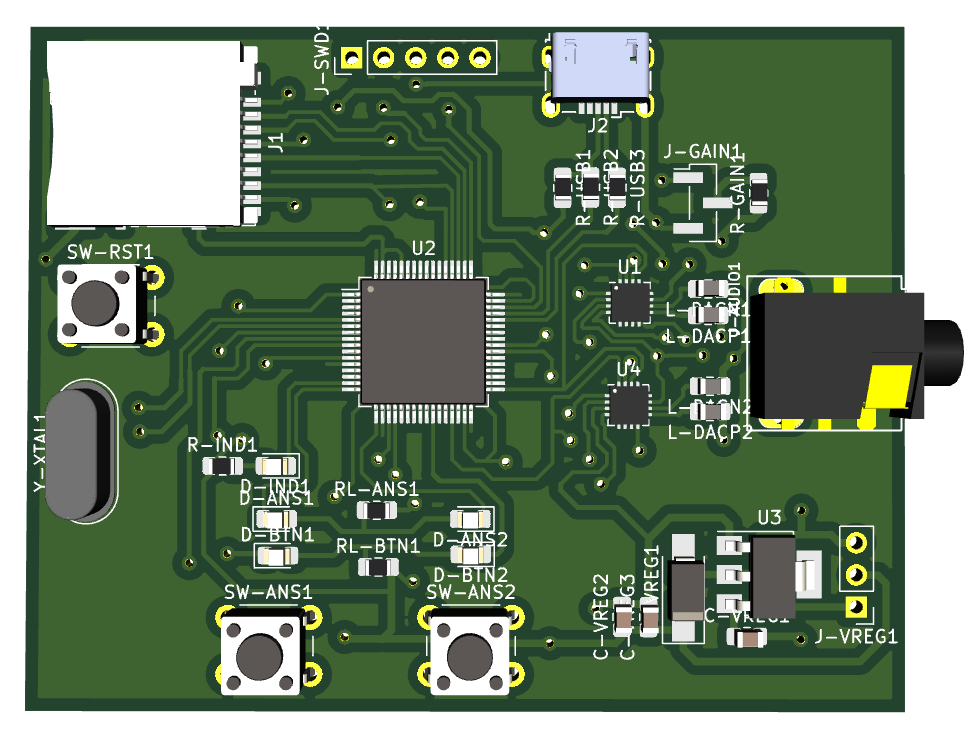
\includegraphics[width=500pt]{images/end_stm32f401re}
	\end{figure}
	
	\vspace*{175pt}
	\noindent This report written using: \\
	OS : \ShowOsVersion \\
	TeX : \ShowTexVersion \\
	Update: {\today} at \currenttime \\

%%%%%%%%%%%%%%%%%%%%%%%%%%%%%%%%%%%%%%%%%%%%%%%%%%%%%%%%%%%%%%%%%	

	\newpage
	\tableofcontents

%%%%%%%%%%%%%%%%%%%%%%%%%%%%%%%%%%%%%%%%%%%%%%%%%%%%%%%%%%%%%%%%%
	
	\newpage
	\section{Completed Design}
	
	Berikut akan dijabarkan desain yang selesai dirakit dan diuji-coba sebagai acuan dasar (\textit{blue-print}).
	
	\subsection{Actual Unit}

	Berikut deskripsi singkat unit yg telah dirakit
	\begin{figure}[!ht]
		\centering
		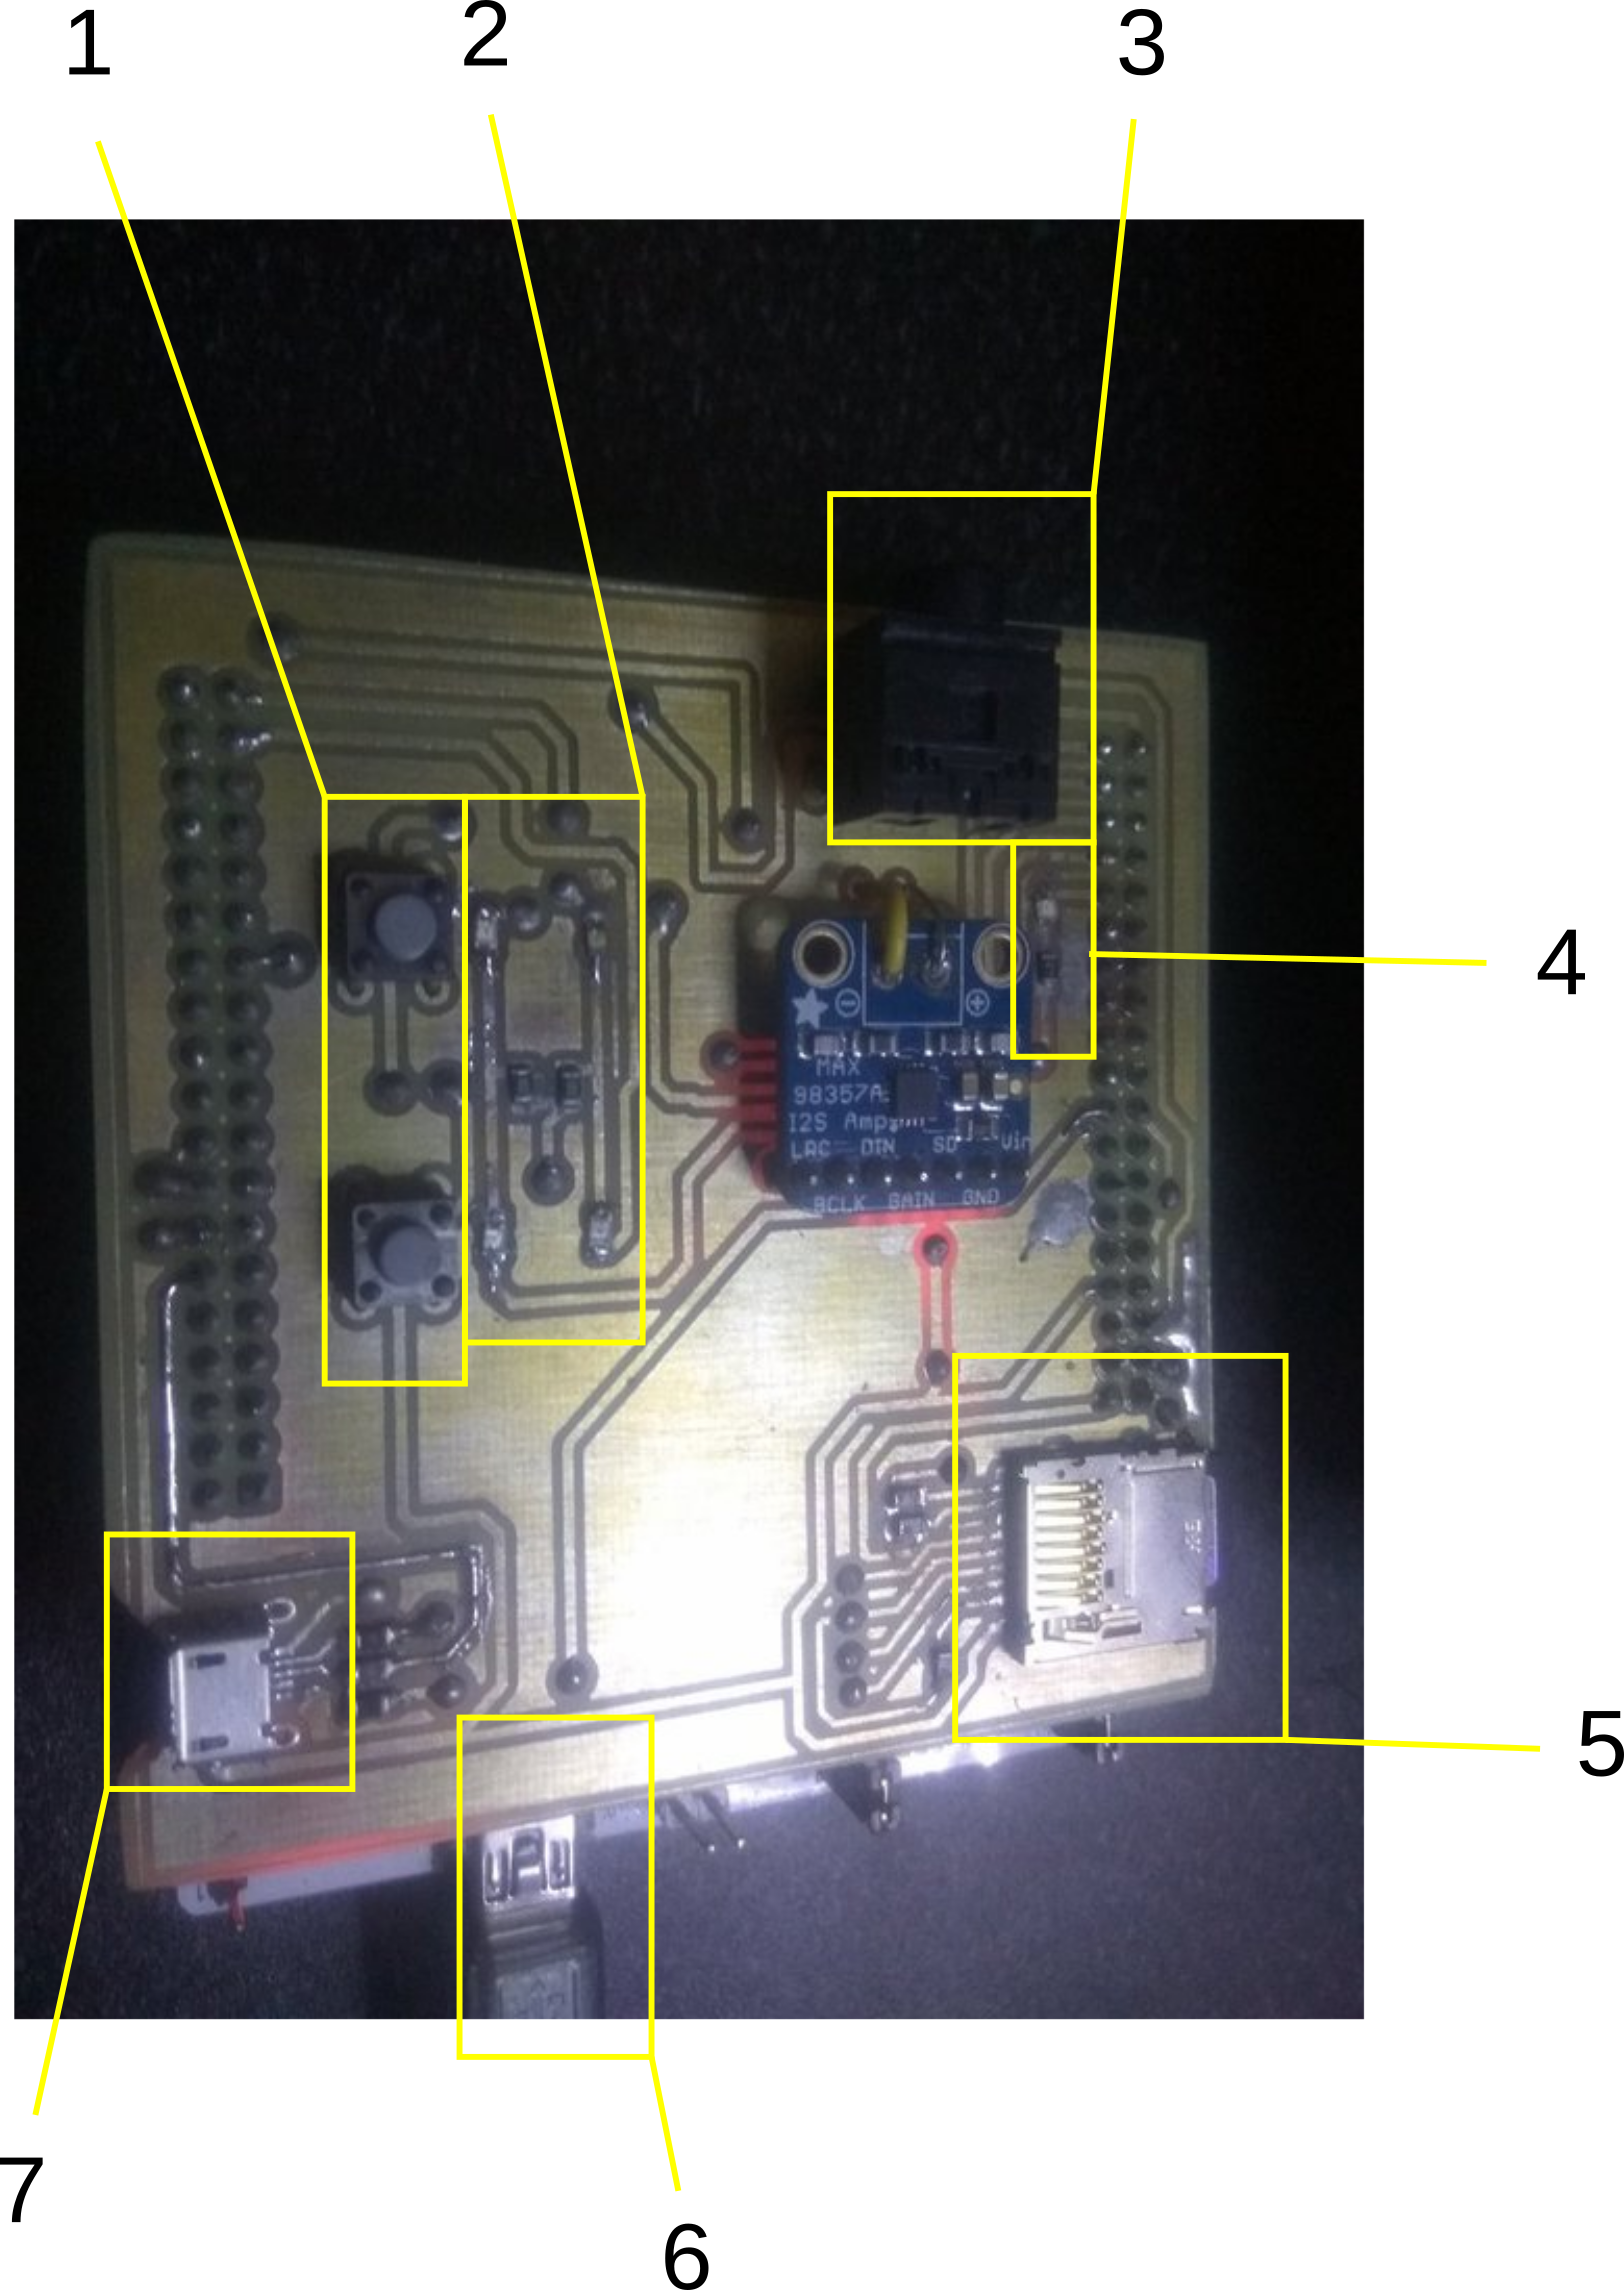
\includegraphics[width=400pt]{images/completed}
		\caption{Actual Unit}
	\end{figure}

	Penjelasan bagian-bagian:
	\begin{enumerate}
		\item Tombol untuk user berinteraksi dengan unit.
		
		\item LED untuk indikator, terdiri dari 2 baris:
		\begin{itemize}
			\item LED indikator jawaban Benar (Hijau) dan Salah (Merah).
			\item LED indikator pilihan jawaban (Kuning) kiri dan kanan sesuai posisi tombol.
		\end{itemize}
	
		\item Jack Audio 3.5mm TRS (Tip-Round-Sleeve) untuk sambungan ke headphone.
		Audio output masih Mono.
		
		\item LED indikator untuk petunjuk mode atau status unit.
		
		\item Soket untuk micro MMC atau SDCard.
		
		\item USB Connector untuk jalur power 5V atau jalur \textit{reprogram} untuk revisi firmware.
		
		\item (Optional) USB Connector untuk jalur komunikasi serial data dengan Android atau komputer.
 
	\end{enumerate}

	\newpage
	\subsection{How To Use}
	
	Berikut dijelaskan secara singkat penggunaan unit Audiometri:
	\begin{enumerate}
		\item Masukkan micro SDCard/MMC berformat FAT32 ke soket MMC/SDCard (nomer 5).
		
		\item Sambungkan Headphone/Earphone ke 3.5mm Audio Jack (nomer 3).
		
		\item Nyalakan unit dengan menyambungkan USB Port (nomer 6) ke sumber tegangan 5v (handphone charger atau power-bank).
		
		\item LED indikator mode (nomer 4) akan menyala berkedip dengan kemungkinan sebagai berikut:
		\begin{itemize}
			\item Berkedip pelan: Unit \textit{ready} dan dalam mode \textit{idle}.
			\item Berkedip cepat dua kali setiap 1.5 detik: Unit error karena MMC/SDCard tidak ada atau error tidak bisa baca-tulis.
			\item LED Mati atau Nyala tidak berkedip: Unit hank/freeze. Matikan unit dan nyalakan ulang.
		\end{itemize}
	
		\item Entering Mode: Standby.\\
		Prosedur:
		\begin{itemize}
			\item Tekan salah satu tombol. LED dekat tombol akan menyala sebagai indikator tombol ditekan.\\
			Tidak ada urutan mana tombol yang perlu dinyalakan lebih dahulu
			
			\item Tekan tombol satu lagi (selain tombol sebelumnya). LED dekat tombol akan mati dan LED hijau nyala.
			
			\item Unit sudah masuk ke mode Standby, subyek uji dipersiapkan.
		\end{itemize}
	
		\begin{figure}[!ht]
			\centering
			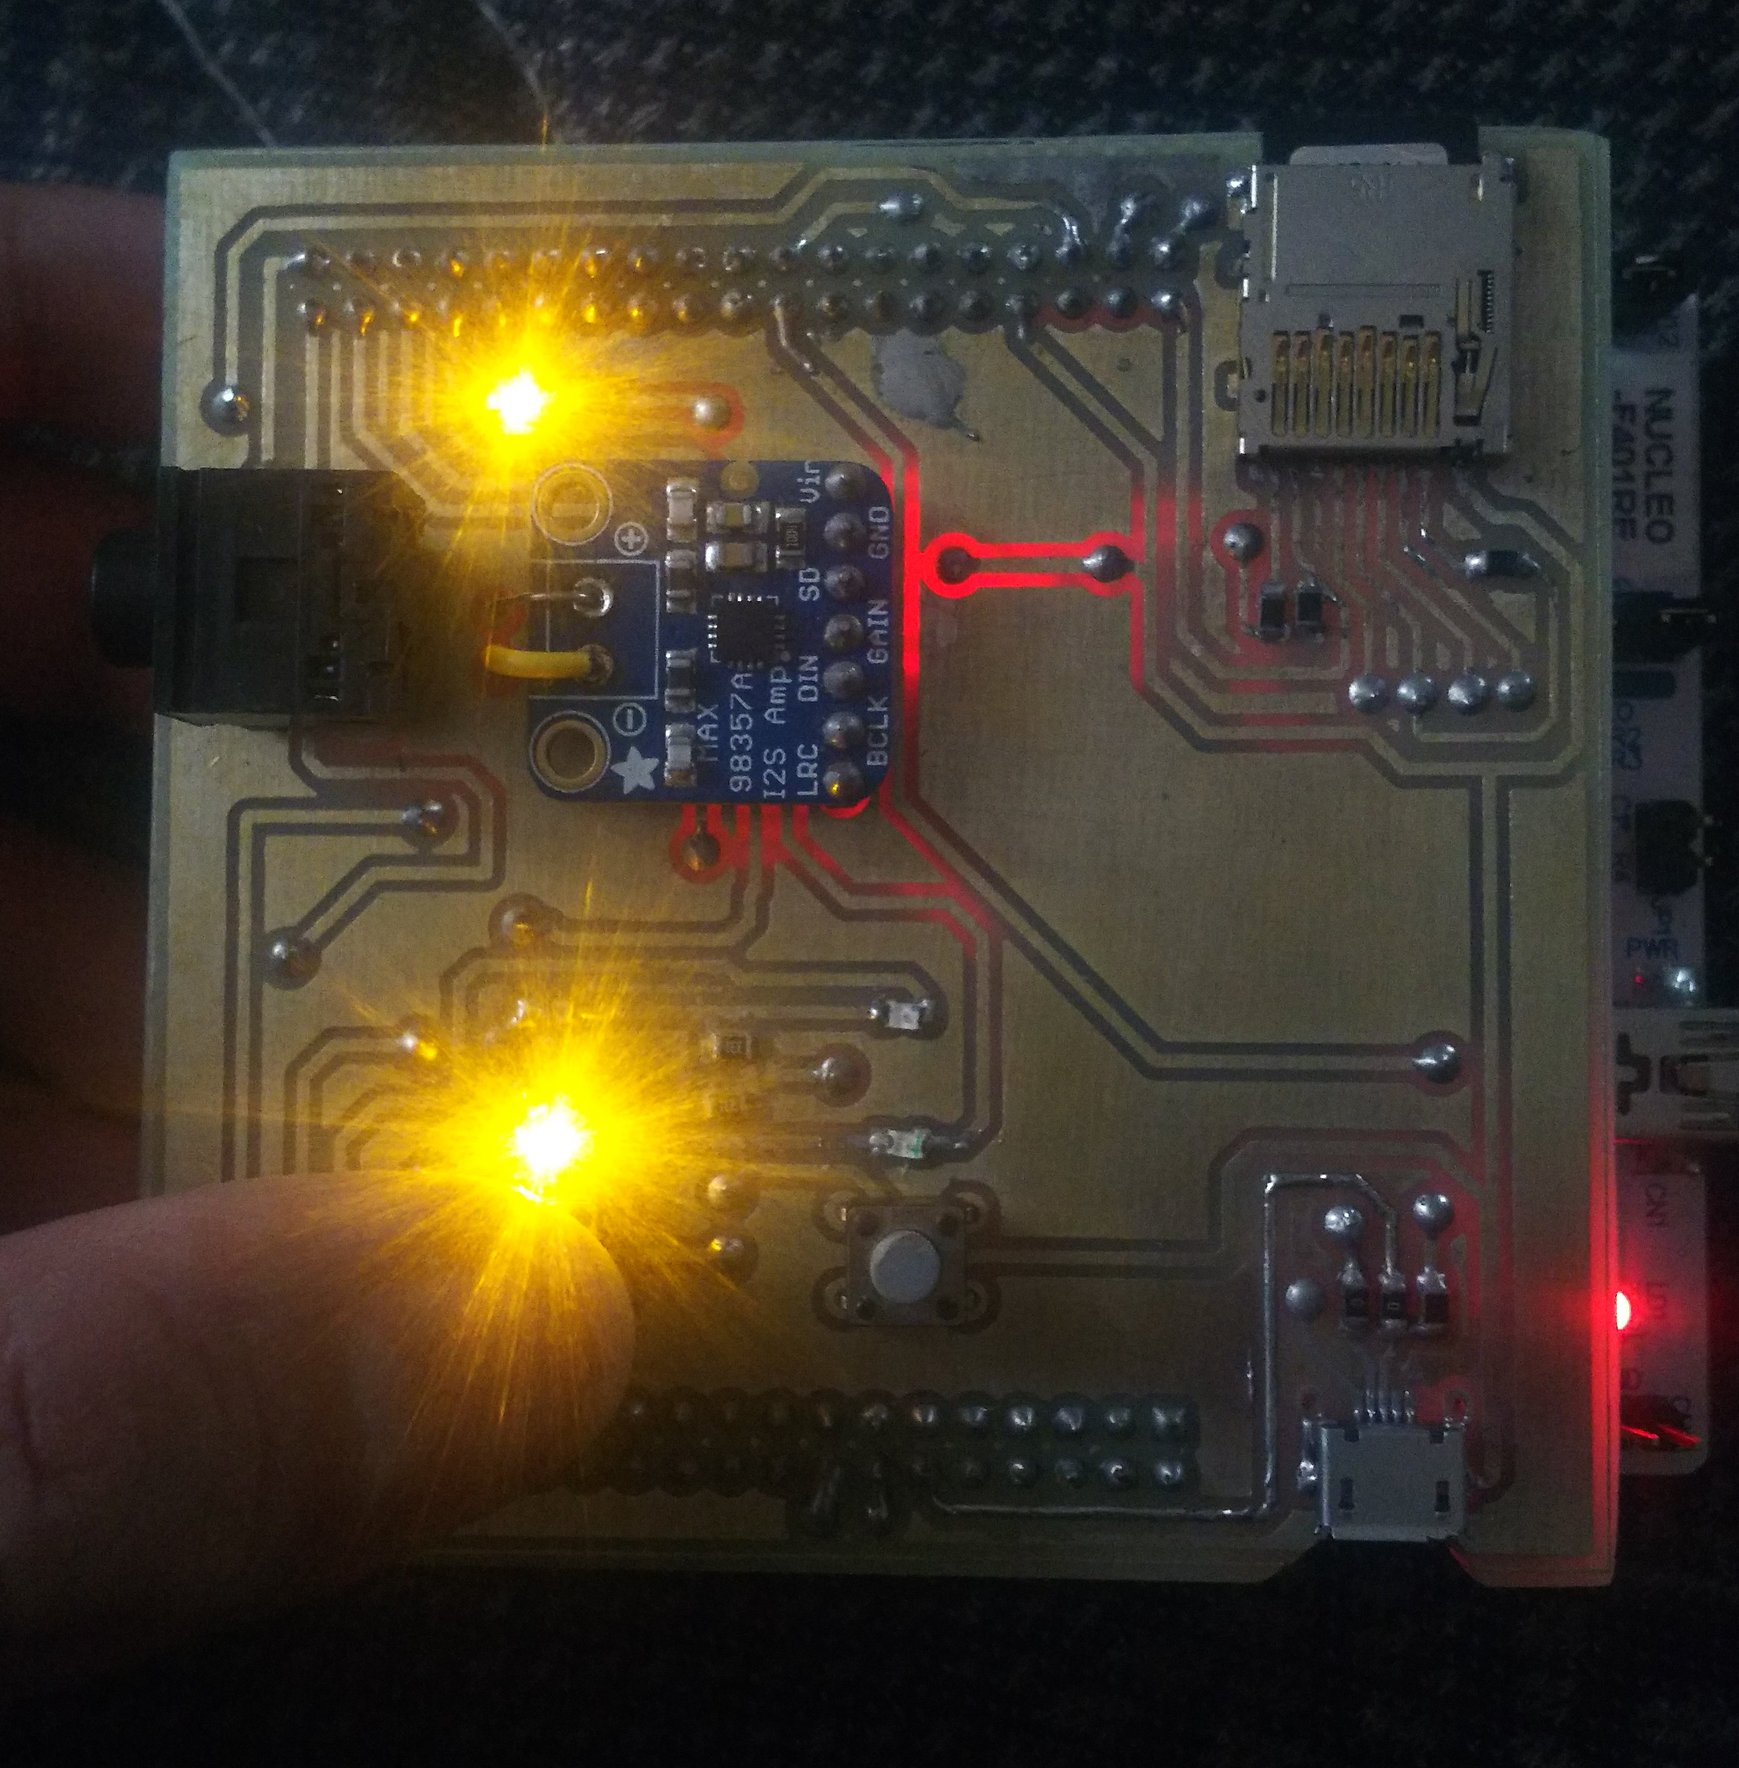
\includegraphics[width=150pt]{images/stndby0}
			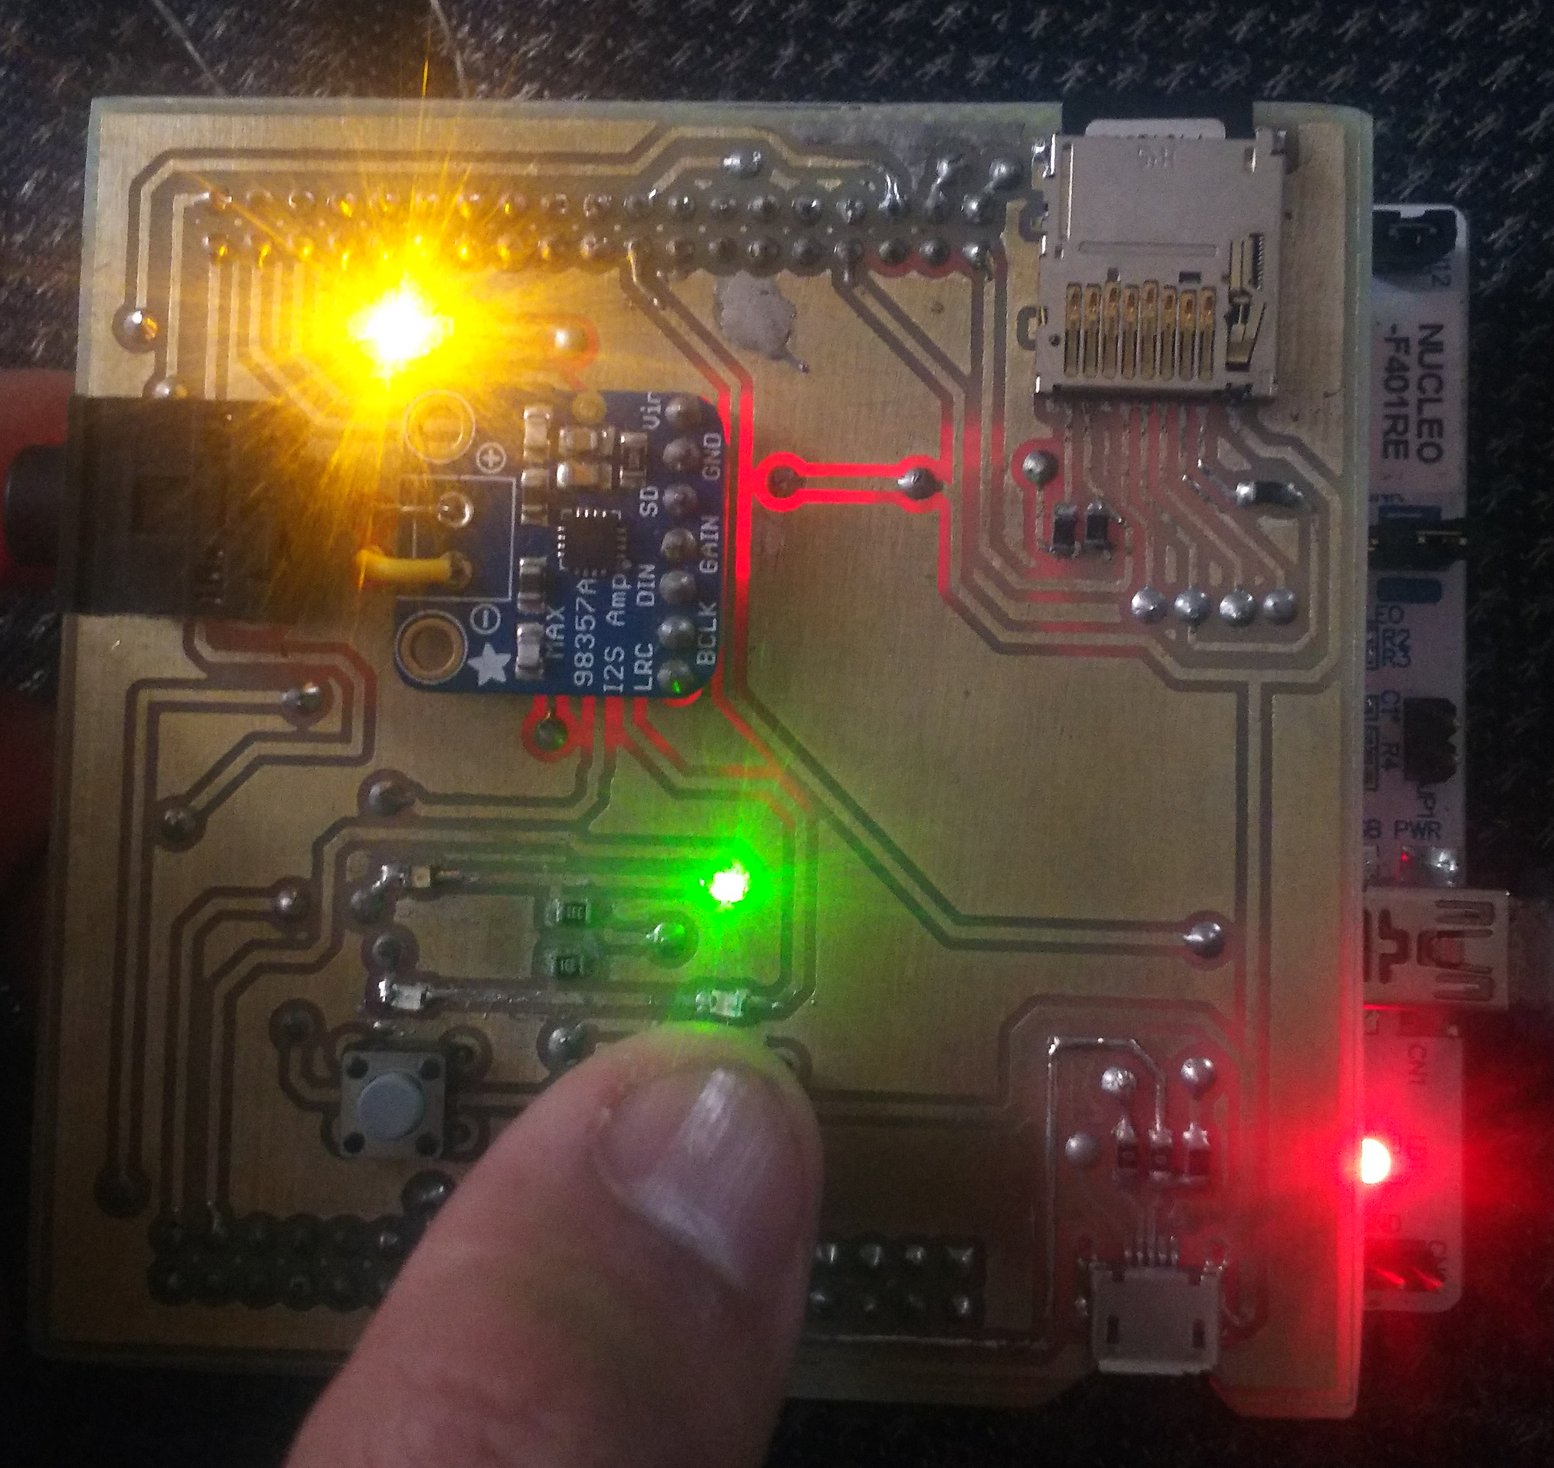
\includegraphics[width=150pt]{images/stndby1}
			\caption{Masuk mode standby (kiri) step pertama dan (kanan) step kedua}
		\end{figure}
	
		\item Entering Mode: Audiometri.\\
		Jika subyek uji sudah siap, maka tinggal tekan salah satu tombol (yang mana saja boleh).\\
		Semua LED akan mati kecuali LED indikator mode (nomer 4) akan berkedip lebih cepat sebagai tanda sudah masuk mode Audiometri.
		
		\item Proses Audiometri:
		Berikut gambaran singkat proses Audiometri:
		\begin{itemize}
			\item LED dekat tombol akan menyala bergantian dengan setiap durasi nyala 1 detik.
			
			\item Unit akan memberikan tone sine-wave berdurasi 1 detik bersamaan dengan salah satu nyala LED.
			
			\item Subyek uji kemudian memilih menekan tombol dimana LED nyala bersamaan dengan mendapat tone dari headphone.
			
			\item Jika benar maka LED Hijau menyala, sebaliknya maka LED Merah menyala.
			
			\item Kemudian 2 detik akan diujikan tone selanjutnya	
		\end{itemize}
		
		\item Selesai proses.
		
		Setelah semua variasi tone diujikan, maka LED indikator mode (nomer 4) akan kembali berkedip pelan sebagai tanda unit kembali ke mode \textit{ready} atau \textit{idle}.
		
		\item Mengambil data record.
		\begin{itemize}
			\item Matikan Unit
			\item Ambil SDCard/MMC dari soket
			\item Masukkan MicroSD Card-Reader
			\item Data bisa disalin di komputer atau handphone
		\end{itemize}
	\end{enumerate}
		
	\newpage
	\subsection{Save File}
	
	Hasil rekaman jawaban subyek uji akan disimpan dalam micro SDCard/MMC dalam format CSV (Comma-Separated Value).
	Nama File menggunakan pola "TEST\_x.TXT" dengan \textbf{x} adalah angka dari 0 sampai 254 dimana angka yang terbesar adalah hasil dari uji yang terakhir.

	Berikut deskripsi ringkas save-file:
	\begin{itemize}
		\item File dimulai dengan \textit{keyword} \textbf{START} dan \textbf{END}.\\
		Save file tanpa salah satu atau kedua keyword ini dianggap invalid.
		
		\item Kolom pertama berisi skala frekuensi, dimana dari hasil uji kalibrasi unit terakhir menunjukkan skala 1 sebanding dengan 485 Hz.\\
		Variasi yang saat ini telah disiapkan adalah 1, 2, 4, 8, 16, dan 32.
		
		\item Kolom kedua berisi skala amplitudo, dimana dari hasil uji kalibrasi unit terakhir menunjukkan skala 1 sebanding dengan 96 dB.
		Variasi yang saat ini telah disiapkan adalah 0.5, 0.25, 0.125, 0.0625, 0.0312, 0.0156, 0.0078, dan 0.0039.
		
		\item Kolom ketiga berisi hasil input jawaban subyek uji Benar atau Salah.
	\end{itemize}
	
	Contoh konten:
	\begin{minted}[frame=lines,framesep=2mm,fontsize=\footnotesize,bgcolor=LightGray]{text}
START
1.00, 0.5000, TRUE
1.00, 0.2500, TRUE
1.00, 0.1250, TRUE
1.00, 0.0625, TRUE
1.00, 0.0312, TRUE
1.00, 0.0156, TRUE
1.00, 0.0078, TRUE
1.00, 0.0039, TRUE
2.00, 0.5000, TRUE
2.00, 0.2500, TRUE
2.00, 0.1250, TRUE
2.00, 0.0625, FALSE
2.00, 0.0312, TRUE
2.00, 0.0156, TRUE
2.00, 0.0078, TRUE
2.00, 0.0039, TRUE
4.00, 0.5000, TRUE
4.00, 0.2500, TRUE
4.00, 0.1250, TRUE
4.00, 0.0625, TRUE
4.00, 0.0312, TRUE
4.00, 0.0156, TRUE
4.00, 0.0078, TRUE
4.00, 0.0039, FALSE
8.00, 0.5000, TRUE
8.00, 0.2500, TRUE
8.00, 0.1250, TRUE
8.00, 0.0625, TRUE
8.00, 0.0312, TRUE
8.00, 0.0156, FALSE
8.00, 0.0078, FALSE
8.00, 0.0039, TRUE
16.00, 0.5000, TRUE
16.00, 0.2500, TRUE
16.00, 0.1250, TRUE
16.00, 0.0625, TRUE
16.00, 0.0312, TRUE
16.00, 0.0156, TRUE
16.00, 0.0078, FALSE
16.00, 0.0039, TRUE
32.00, 0.5000, TRUE
32.00, 0.2500, TRUE
32.00, 0.1250, TRUE
32.00, 0.0625, TRUE
32.00, 0.0312, TRUE
32.00, 0.0156, TRUE
32.00, 0.0078, TRUE
32.00, 0.0039, TRUE
END
	\end{minted}
	
	\newpage
	\subsection{Need to be defined}
	
	Berikut adalah beberapa poin yang perlu ditinjau lebih jauh sebelum \textit{blueprint} dianggap siap:
	
	\begin{itemize}
		\item Randomness dari pilihan jawaban.\\
		Untuk membuat pilihan jawaban antara tombol kiri dan kanan, digunakan algoritma \textit{pseudo-random}
		untuk generate random number antara 0 hingga 50, kemudian posisi jawaban tone yang benar ditentukan oleh
		bilangan yang muncul ganjil atau genap.\\
		Mengingat pseudo-random disini hanya menggunakan \textit{seed} konstan dan bukan hardware-based,
		maka tingkat randomness nya belum bisa dianggap tinggi (meragukan).
		
		\item Convinient Level.\\
		Mengingat randomness yang masih diragukan, kemudian ditambah setiap pasangan
		variasi frekuensi dan amplitudo hanya sekali diujikan pada subyek uji, 
		maka bisa diduga hasilnya mungkin tidak representatif dan tidak konsisten terhadap satu obyek uji.\\
		Perlu metode pungujian baru terhadap subyek berdasarkan \textit{convinient-level},
		sehingga perlu ada definisi matematis atau programatikal untuk convinient-level tersebut. 
		
		\item Actual dB.\\
		Berdasarkan datasheet, output dari DAC MAX98357A adalah sebagai berikut:
		
		\[S_o = S_i + A_g + A_c\]
		
		dimana:
		\begin{itemize}
			\item $S_o$ adalah signal output (dBV)
			\item $S_i$ adalah signal input (dBFS)
			\item $A_g$ adalah audio gain (dB)
			\item $A_c$ adalah minimum output (2.1 dB)
		\end{itemize}
		
		Mengingat konversi dBV ke audio dB secara matematis sangat bergantung dengan tipe dan impedansi headphone atau earphone,
		maka perlu disepakati standar tipe atau impedansi headphone/earphone yang akan digunakan hingga produk akhir nanti. 
		
		\item Audiometri Standard.
		Terakhir yang perlu didefinisikan adalah standar audiometri yang akan digunakan sehingga mudah untuk implementasi secara programatikal,
		yang nantinya digunakan sebagai acuan target kalibrasi.
		
		Meliputi setidaknya:
		\begin{itemize}
			\item Standar frekuensi 			
			\item Standar SPL yang sesuai audiometri
			\item Standar durasi per tone
		\end{itemize}
	\end{itemize}

	Apabila telah jelas terdefinisi poin-poin tersebut, maka blueprint dianggap siap.
	Selanjutnya adalah tinggal merancang \textit{packanging}, mengajukan sertifikasi, dan merencanakan proses fabrikasi massal.
	
	\newpage
	\section{Next Development}
	
	Berikut akan dijabarkan ringkas terkait hasil dan kebutuhan pengembangan versi selanjutnya dimana
	diharapkan menjadi MVP (Minimum Viable Product) yang siap dibuat dalam jumlah terbatas.
	Perlu diingat bahwa apa yang dijabarkan disini masih berasumsi pada proses manufaktur kecil
	dan belum melakukan kontrak dengan pihak manufaktur mana pun.
	
	\subsection{Circuit Board}
	
	Untuk produksi PCB, disini telah dipilih CV Maxtron Persada Indonesia dengan kantor beralamat di HCC Trosobo, Sidoarjo.
	Pertimbangan memilih adalah:
	\begin{itemize}
		\item Manufaktur lokal yang tidak terlalu jauh dengan area kampus ITS.
		\item Harga cukup terjangkau dan bisa order tanpa minimum batch dan
		hanya mewajibkan minimal luas PCB adalah 100$cm^2$ dengan harga kisaran Rp.100.000,- per biji.
		\item Kualitas hasil fabrikasi tergolong bagus untuk PCB-fiber dengan requirement 
		double-layer, pin-through-hole, thin-mask, dan wire-line ukuran hingga 0.25mm. 
	\end{itemize}

	\begin{figure}[!ht]
		\centering
		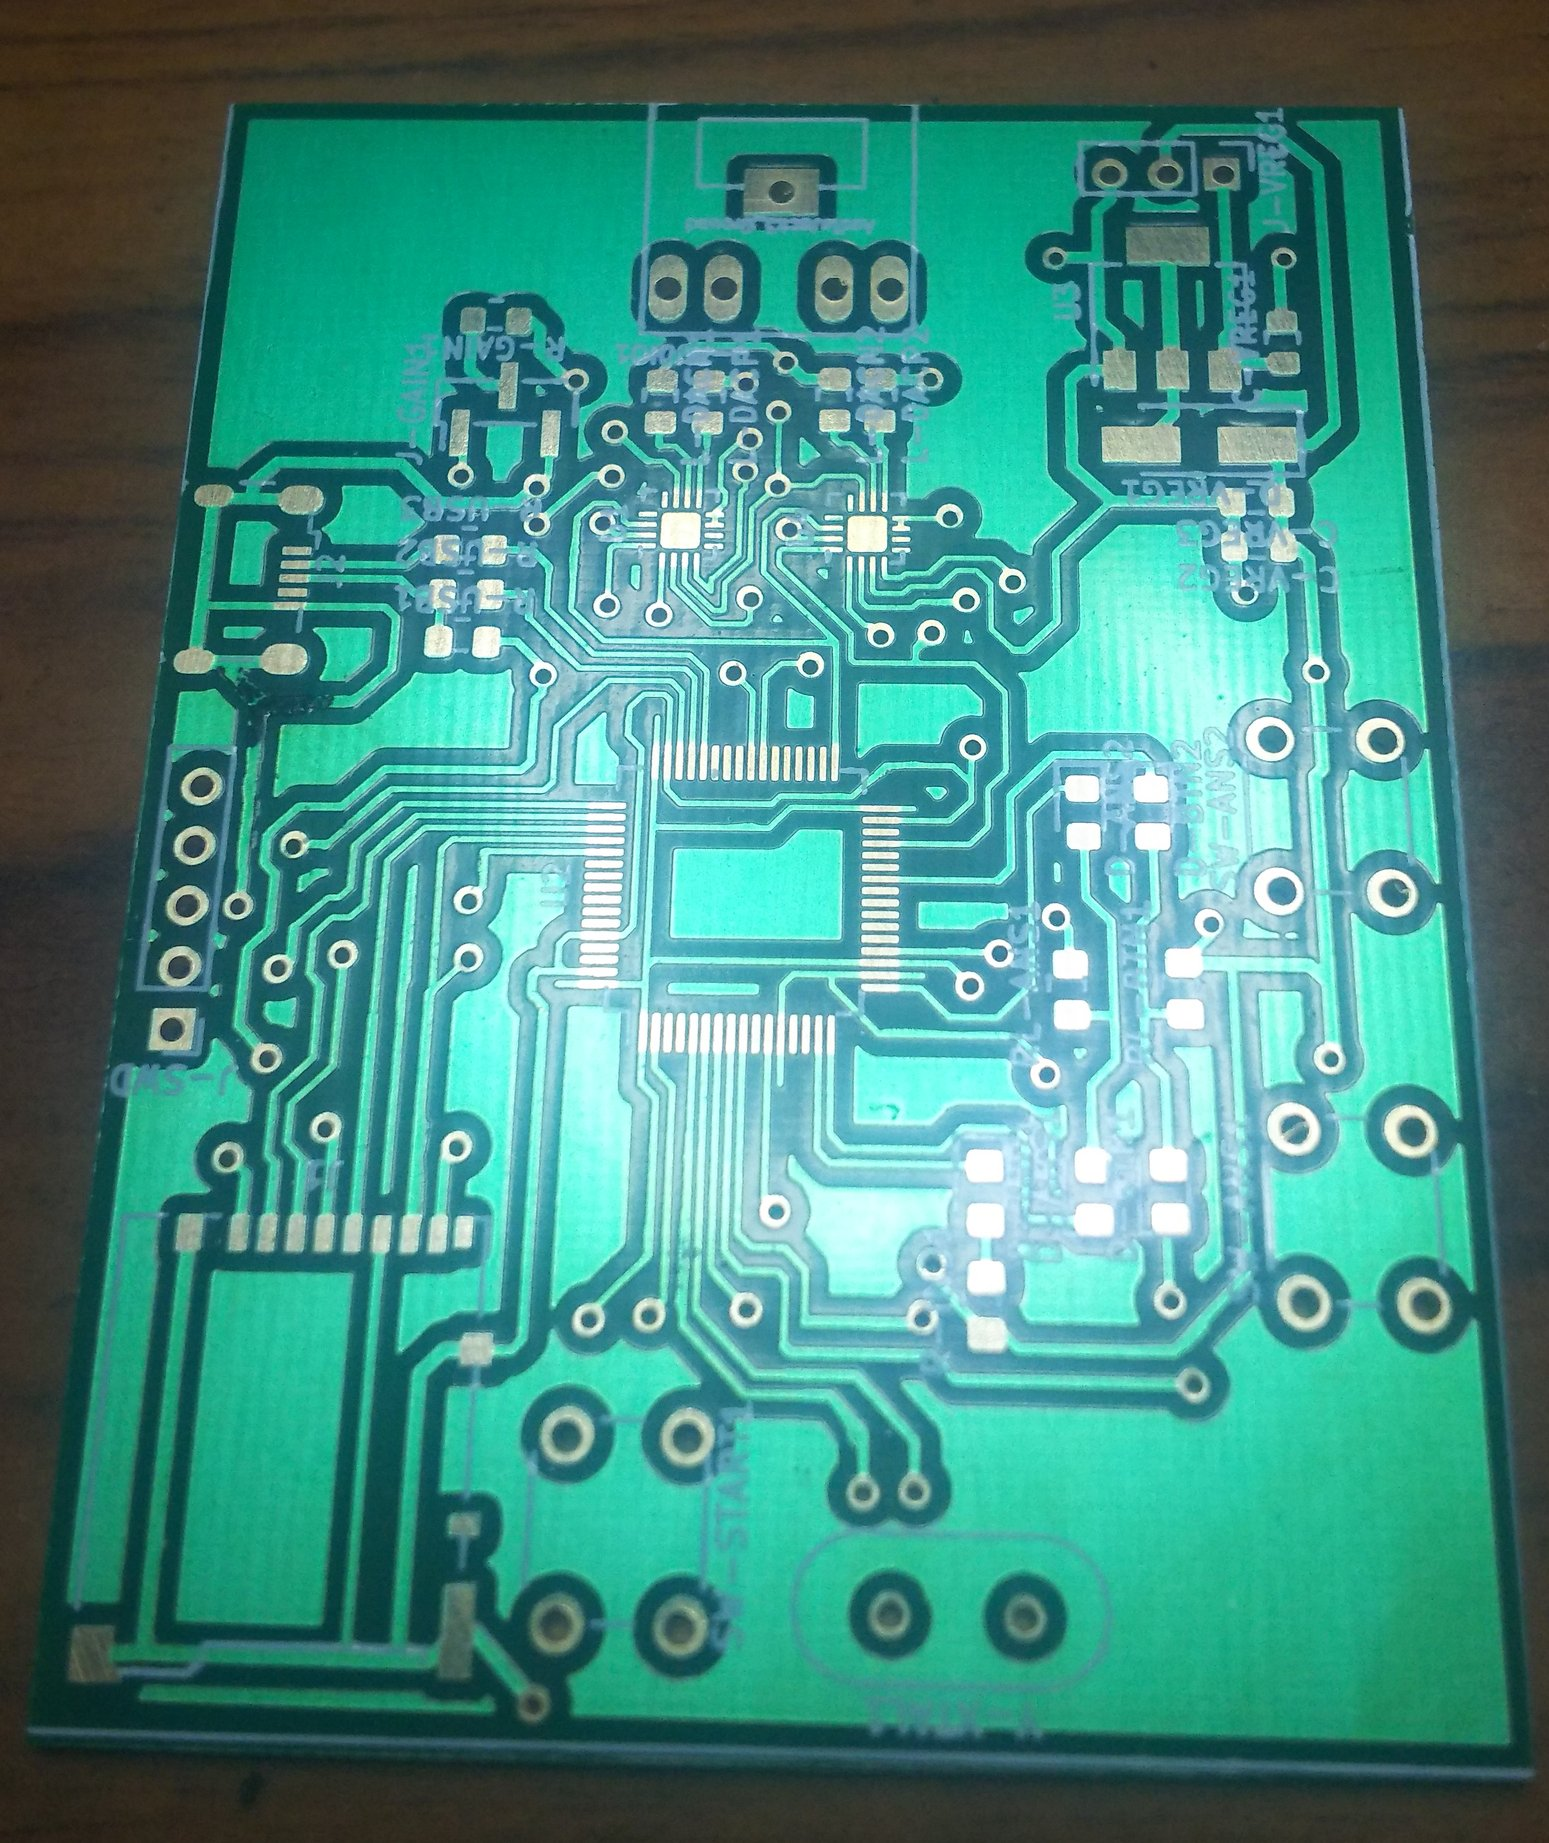
\includegraphics[width=300pt]{images/pcb}
		\caption{PCB hasil fabrikasi}
	\end{figure}

	\newpage
	\subsection{Components Purchasing}    
	
	Berdasarkan pantauan di lapangan, seller komponen eletronik raw (non-module) semakin menipis,
	mengingat profit penjualan komponen raw memang jauh lebih kecil dibandingkan penjualan dalam modul.
	
	Untuk itu, diputuskan melakukan pengadaan (impor) paket/batch komponen sendiri.
	Berikut daftar komponen utama yang perlu diimpor:
	
	\begin{itemize}
		\item STM32F401RET6
		\begin{itemize}
			\item Price: \$25.18
			\item Qty: 10
			\item ETA: 20-35 days
			\item URL: \url{https://id.aliexpress.com/item/33016842828.html}
		\end{itemize}
	
		\item MAX98357A
		\begin{itemize}
			\item Price: \$16.61
			\item Qty: 10
			\item ETA: 20-35 days
			\item URL: \url{https://id.aliexpress.com/item/32953327741.html}
		\end{itemize}
	
		\item MicroSD Connecttor
		\begin{itemize}
			\item Price: \$3.60/piece
			\item Qty: 5
			\item Total: \$18
			\item ETA: 20-35 days
			\item URL: \url{https://id.aliexpress.com/item/32911089040.html}
		\end{itemize}
	
		\item LED 0805
		\begin{itemize}
			\item Price: \$1.49/reel
			\item Qty: 3 
			\item Total: \$4.47
			\item ETA: 24-44 days
			\item URL: \url{https://id.aliexpress.com/item/32320996015.html}
		\end{itemize}
	
		\item Battery Regulator TP4056
		\begin{itemize}
			\item Price: \$2.99
			\item Qty: 5
			\item Total: \$18
			\item ETA: Sebelum 25 April atau dana kembali 
			\item URL: \url{https://id.aliexpress.com/item/4000196554965.html}
		\end{itemize}
	
		\item Battery LiPO 3.7v 300mAh
		\begin{itemize}
			\item Price: \$1.79
			\item Qty: 5
			\item Total: \$8.95
			\item ETA: Sebelum 21 April atau dana kembali 
			\item URL: \url{https://id.aliexpress.com/item/32956465921.html}
			\item Catatan: Battery dan device dengan baterry sering dianggap bukan komponen raw,
			sehingga ada kemungkinan tambahan pajak cukai.
		\end{itemize}
	
	\end{itemize}
		
\end{document}